
\begin{center}

\includegraphics[width=0.7\textwidth]{content/3/chapter4/images/2.png}\\
\end{center}

为了充分理解概念,需要先了解概念出现的原因。

\subsubsubsection{4.1.1\hspace{0.2cm}两种错误的方法}

C++20之前,可以有两种截然相反的方式来思考函数或类:为特定类型或泛型类型定义。后者,称之为函数模板或类模板。不过,这两种方法都有各自的问题:

\hspace*{\fill} \\ %插入空行
\noindent
\textbf{4.1.1.1\hspace{0.2cm}太具体}

为每种类型的重载函数,或是重新进行类实现是一项乏味的工作。为了避免这种重复,通常会使用类型转换。不过,这种方式看似拯救,却又是诅咒。

\hspace*{\fill} \\ %插入空行
\noindent
\textbf{类型的隐式转换}
\begin{lstlisting}[style=styleCXX]
// tooSpecific.cpp

#include <iostream>

void needInt(int i){
	std::cout << "int: " << i << '\n';
}

int main(){

	std::cout << std::boolalpha << '\n';

	double d{1.234};
	std::cout << "double: " << d << '\n';
	needInt(d);

	std::cout << '\n';

	bool b{true};
	std::cout << "bool: " << b << '\n';
	needInt(b);

	std::cout << '\n';

}
\end{lstlisting}

例子(第13行)以double开始,以int结束(第15行)。第二次,以bool开始(第19行),并以int结束(第21行)。

\begin{center}
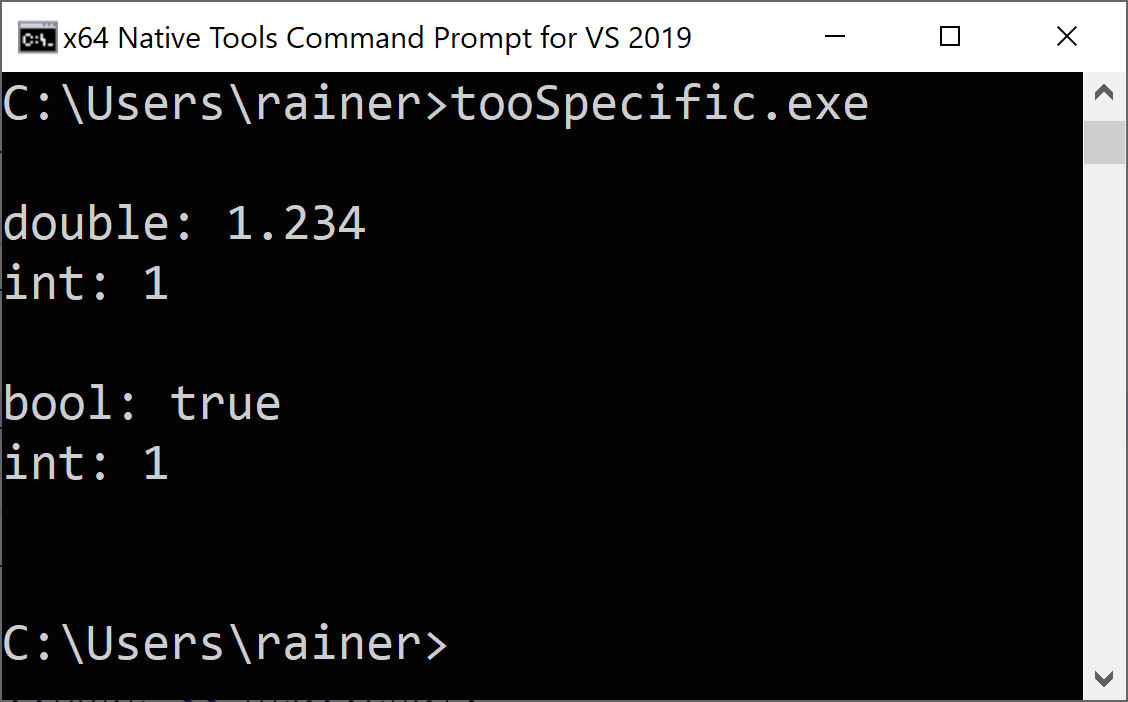
\includegraphics[width=0.6\textwidth]{content/3/chapter4/images/3.png}\\
\end{center}

例子进行了两次类型隐式转换。

\hspace*{\fill} \\ %插入空行
\noindent
\textbf{4.1.1.1.1\hspace{0.2cm}窄化转换}

使用double类型调用getInt(int a)可以实现窄化转换。窄化转换是一种类型转换,包括精度损失。但有时,开发者并不想有任何损失。

\hspace*{\fill} \\ %插入空行
\noindent
\textbf{4.1.1.1.2\hspace{0.2cm}类型提升}

反过来会更好吗?

使用bool类型调用getInt(int a),可将bool类型提升为int类型。惊讶吗?许多C++开发人员在添加两个bool时,并不知道他们会得到的是哪种数据类型。

\hspace*{\fill} \\ %插入空行
\noindent
\textbf{对两个布尔值进行加法运算}
\begin{lstlisting}[style=styleCXX]
template <typename T>
auto add(T first, T second){
	return first + second;
}

int main(){
	add(true, false);
}
\end{lstlisting}

\href{https://cppinsights.io/s/9bd14f99}{C++ Insights}在编译器在实例化中转换函数模板后,并将上面的源代码可视化。

\begin{center}
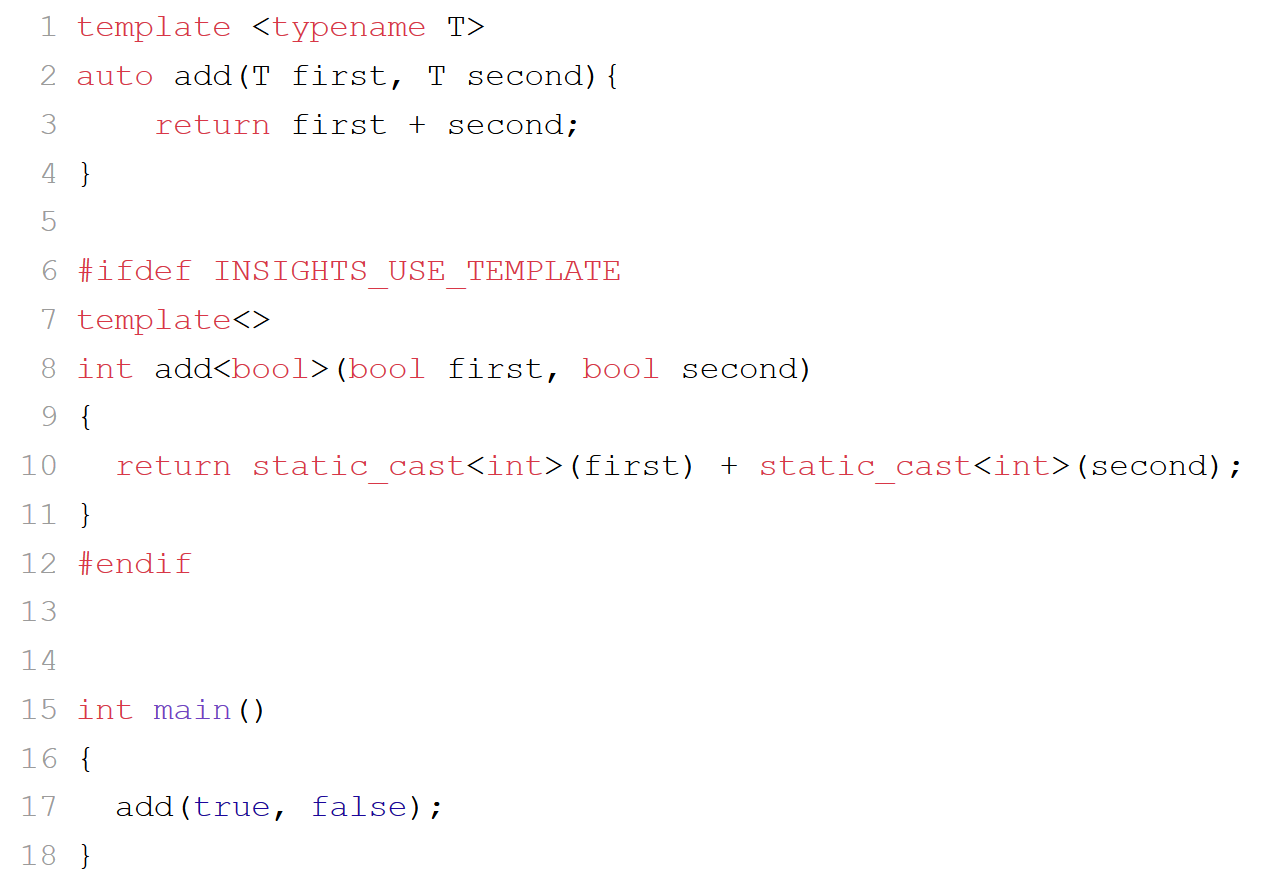
\includegraphics[width=0.8\textwidth]{content/3/chapter4/images/1-1.png}\\
bool提升为int
\end{center}

第8-14行是\href{https://cppinsights.io/}{C++ Insights}截图中的关键行。函数模板add的模板实例化,使用返回类型int创建一个全特化函数,从而两个bool类型的参数都隐式提升为int。

因为我们不想为每种类型重载函数或重新实现类,来尝试依赖于转换的魔力。

让我试试另一种方式,用一个泛型函数。

\hspace*{\fill} \\ %插入空行
\noindent
\textbf{4.1.1.2\hspace{0.2cm}太通用}

容器排序是一个很普遍的需求。若容器的元素支持排序,那么就应该适用于每个容器。下面的示例中,我将标准算法std::sort应用于标准容器std::list。

\hspace*{\fill} \\ %插入空行
\noindent
\textbf{对std::list排序}
\begin{lstlisting}[style=styleCXX]
// tooGeneric.cpp

#include <algorithm>
#include <list>

int main(){

	std::list<int> myList{1, 10, 3, 2, 5};

	std::sort(myList.begin(), myList.end());

}
\end{lstlisting}

\begin{center}
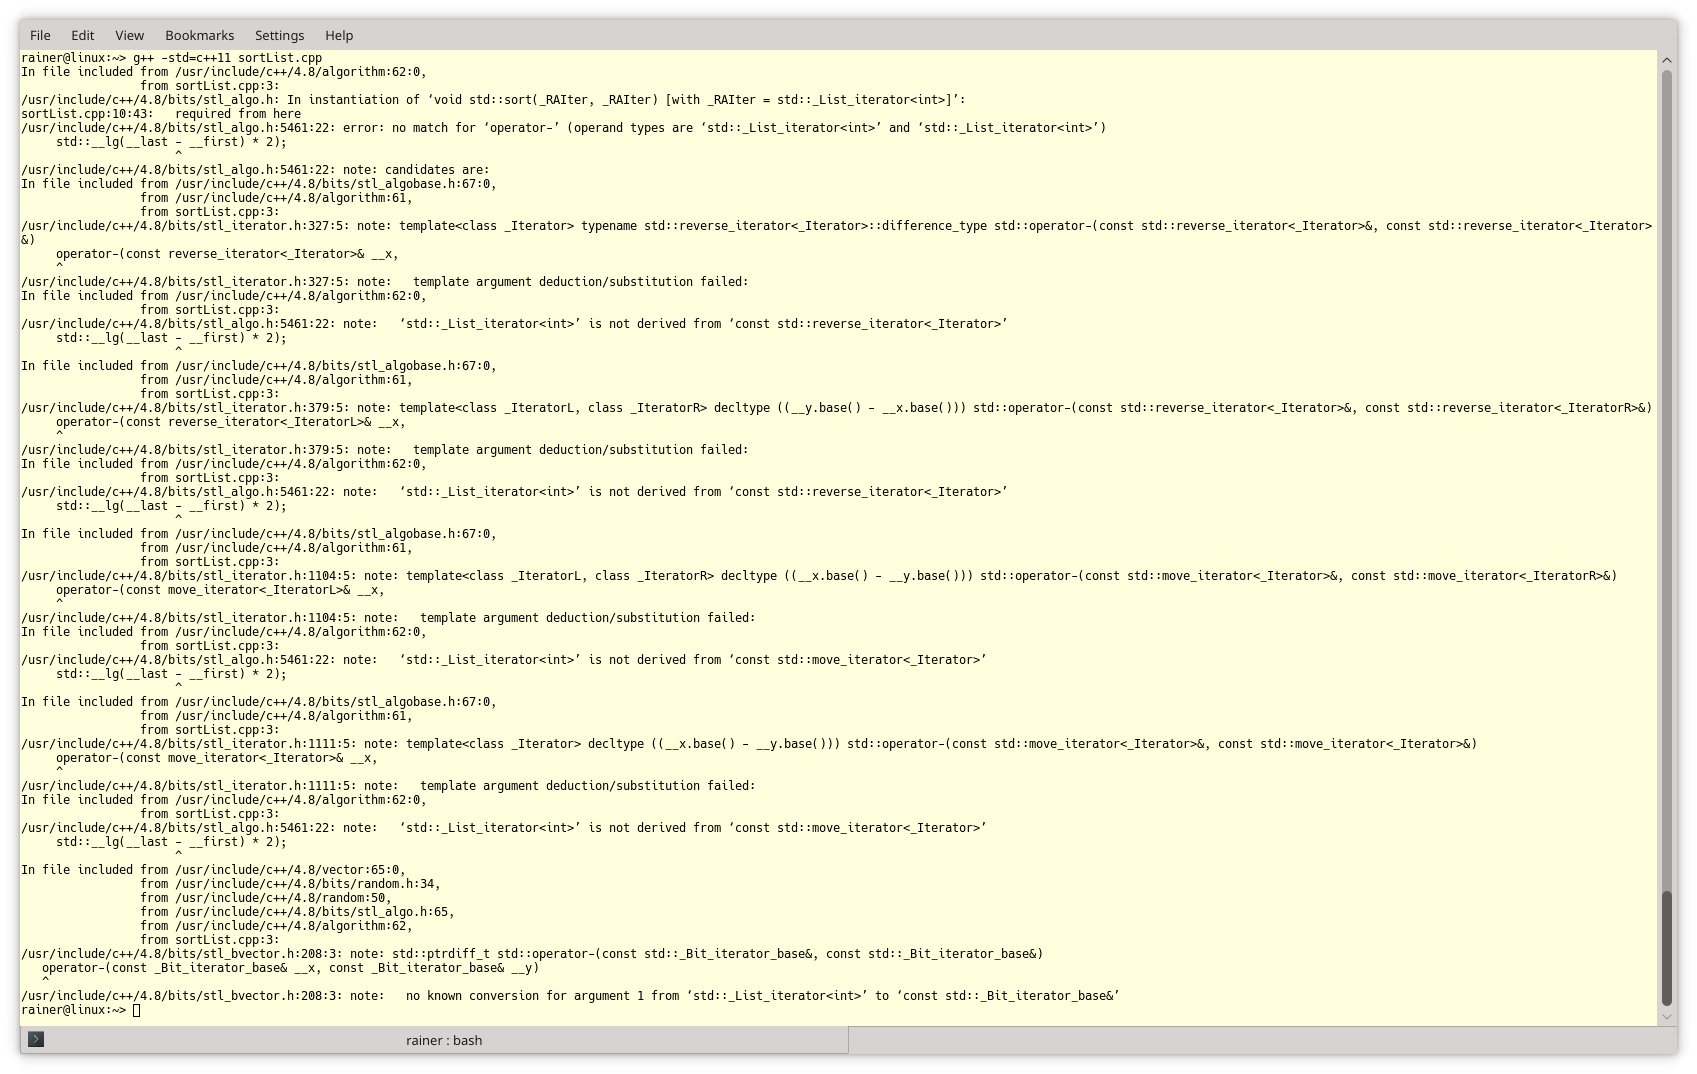
\includegraphics[width=1.0\textwidth]{content/3/chapter4/images/4.png}\\
对std::list进行排序时,编译器报错
\end{center}

我不想解析这么长的信息,但还是要看看出什么问题了。看一下本例中使用的\href{https://en.cppreference.com/w/cpp/algorithm/sort}{std::sort}特定重载的签名。

\hspace*{\fill} \\ %插入空行
\begin{lstlisting}[style=styleCXX]
template< class RandomIt >
constexpr void sort( RandomIt first, RandomIt last );
\end{lstlisting}

std::sort使用了奇怪的参数类型RandomIt。RandomIt代表随机访问迭代器,也就是编译错误提供的关键信息。std::list只提供双向迭代器,但std:sort需要一个随机访问迭代器。下图显示了为什么std::list不支持随机访问迭代器。

\begin{center}

\includegraphics[width=0.8\textwidth]{content/3/chapter4/images/5.png}\\
\end{center}

去看一下cppreference.com上的std::sort文档,会发现一些模板参数对类型有要求。它们对类型提出了概念性的要求,这些要求形成了C++20的概念。

\hspace*{\fill} \\ %插入空行
\noindent
\textbf{4.1.1.3\hspace{0.2cm}概念}

概念对模板参数施加语义约束,std::sort具有接受比较器的重载。

\begin{lstlisting}[style=styleCXX]
template< class RandomIt, class Compare >
constexpr void sort(RandomIt first, RandomIt last, Compare comp);
\end{lstlisting}

下面是std::sort重载的类型要求:

\begin{itemize}
\item
RandomIt必须满足ValueSwappable和LegacyRandomAccessIterator的要求

\item
解引用RandomIt的类型必须满足MoveAssignable和MoveConstructible的要求。

\item
可解引用的RandomIt的类型必须满足Compare的要求。
\end{itemize}

ValueSwappable或LegacyRandomAccessIterator之类的要求就是类型需求,其中一些需求在C++20的\href{https://en.cppreference.com/w/cpp/language/constraints}{概念}中形式化了。

并且,std::sort还需要一个LegacyRandomAccessIterator,在C++20中称为random\_access\_iterator(是<iterator>的一部分):

\hspace*{\fill} \\ %插入空行
\noindent
\textbf{std::random\_access\_iterator}
\begin{lstlisting}[style=styleCXX]
template<class I>
	concept random_access_iterator =
		bidirectional_iterator<I> &&
		derived_from<ITER_CONCEPT(I), random_access_iterator_tag> &&
		totally_ordered<I> &&
		sized_sentinel_for<I, I> &&
		requires(I i, const I j, const iter_difference_t<I> n) {
			{ i += n } -> same_as<I&>;
			{ j + n } -> same_as<I>;
			{ n + j } -> same_as<I>;
			{ i -= n } -> same_as<I&>;
			{ j - n } -> same_as<I>;
			{ j[n] } -> same_as<iter_reference_t<I>>;
		};
\end{lstlisting}

类型I支持概念random\_access\_iterator,若支持概念bidirectional\_iterator和以下所有需求。例如,\{i += n\} \texttt{->} same\_as<I\&>作为需求表达式的一部分,意味着对于类型为i的值,\{i += n\}是一个有效的表达式,返回类型为I\&。对于链表,std::list支持的是bidirectional\_iterator,而非std::sort要求的random\_access\_iterator。

现在需要random\_access\_iterator的算法,接收到birectional\_iterator时,就会显示一条简洁易懂的错误消息,明确的表示迭代器不满足random\_access\_iterator的要求。

\begin{center}
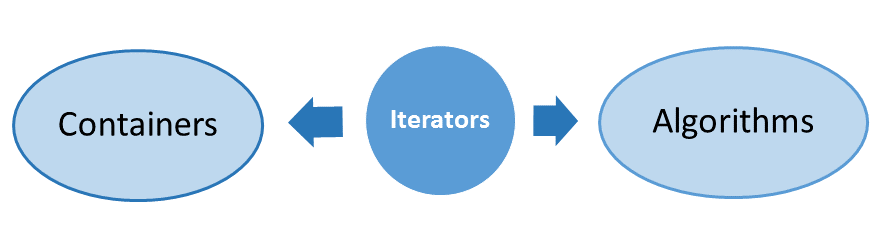
\includegraphics[width=0.7\textwidth]{content/3/chapter4/images/6.png}\\
标准模板库
\end{center}

\begin{tcolorbox}[breakable,enhanced jigsaw,colback=blue!5!white,colframe=blue!75!black,title={泛型编程的本质}]
我想引用Alexander Stepanov(标准模板库的创建者)和Daniel Rose(信息检索研究员)写的书\href{https://www.fm2gp.com/}{《From Mathematics to Generic Programming》}中的一段话来开始这段简短的回顾:“泛型编程的本质在于概念的思想,概念是描述一系列相关对象类型的一种方式。”这些相关的对象类型可以是整型,如bool、char或int。概念是对相关类型的一组需求,例如:所支持的操作、语义,以及时间和空间的复杂度。

\hspace*{\fill} \\ %插入空行
标准模板库(STL)作为一个基于概念的通用库,由三个部分组成:容器,运行在容器上的算法,以及连接它们的迭代器。

\hspace*{\fill} \\ %插入空行
每个容器都提供了符合其结构的迭代器,算法可以对这些迭代器进行操作。容器(如序列容器或关联容器)基于半开放范围模型。迭代器提供对容器元素的访问,并且可以遍历容器,从而可对其进行比较。STL的抽象基于半开放范围模型和迭代器等概念,从而可以使用STL的容器和算法。
\end{tcolorbox}

那么,概念的优势是什么?

\subsubsubsection{4.1.2\hspace{0.2cm}概念的优势}

\begin{itemize}
\item
模板参数的需求描述是接口声明的一部分。

\item
函数的重载和类模板的特化可以基于概念。

\item
概念可用于函数模板、类模板和类或类模板的泛型成员函数。

\item
因为编译器会将模板形参的要求与给定的模板实参进行比较,所以可得到明确的错误消息。

\item
可以使用预定义的概念,也可以自定义概念。

\item
auto和概念的用法统一,可以用概念来代替auto。

\item
若函数声明使用了概念,则它自动成为函数模板。因此,编写函数模板就会如同编写函数一样简单。
\end{itemize}


\subsubsubsection{4.1.3\hspace{0.2cm}漫长的历史}

我第一次听说概念是在2005 - 2006年左右,这让我想起Haskell的课程,Haskell类型就具有类似的接口。下面是\href{https://en.wikipedia.org/wiki/Haskell_(programming_language)}{Haskell的}类型类层次结构的一部分。

\begin{center}
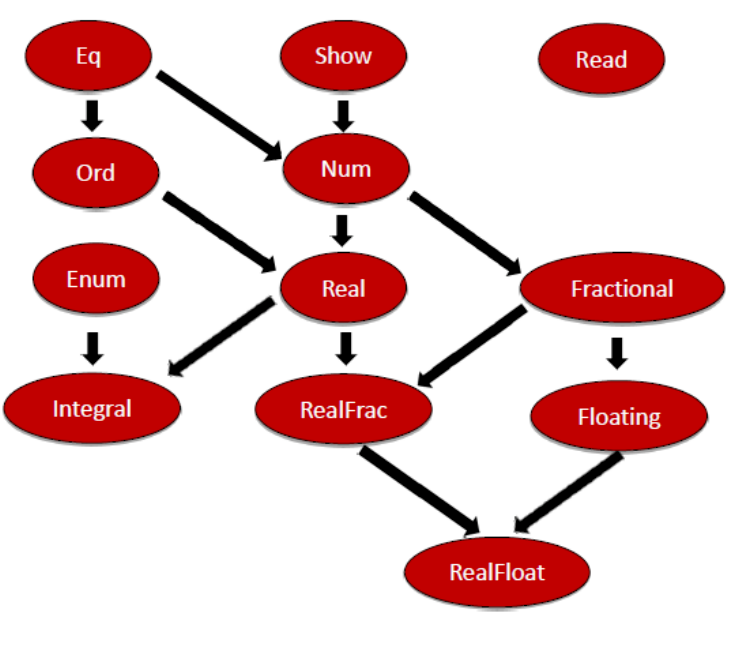
\includegraphics[width=0.8\textwidth]{content/3/chapter4/images/7.png}\\
Haskell类型的层次结构
\end{center}

但C++的概念不同。以下是我观察到的结果。

\begin{itemize}
\item
Haskell中,类型都必须是实例。C++20中,类型必须满足概念的需求。

\item
C++中,概念可以用在模板的非类型参数上。例如,像值5这样的数字就是非类型参数。例如,当想要一个包含5个元素的整型数组std::array时,可以使用非类型参数5:std::array<int, 5> myArray。

\item
概念不会增加运行时的成本。
\end{itemize}

最初,概念是C++11的关键特性,但在2009年7月法兰克福的标准化会议上删除了。这里引用Bjarne Stroustrup对当时概念的看法:\href{https://isocpp.org/blog/2013/02/concepts-lite-constraining-templates-with-predicates-andrew-sutton-bjarne-s}{“C++0x的概念变成一个复杂的怪物”}。几年后,第二次尝试也没有成功:精简版概念从C++17标准中删除了。最终,成了C++20的一部分。

\subsubsubsection{4.1.4\hspace{0.2cm}概念的使用}

可以用四种方式来概念。

\hspace*{\fill} \\ %插入空行
\noindent
\textbf{4.1.4.1\hspace{0.2cm}四种方式}

我在conceptsintegralvariables.cpp中演示了这四种方式,使用了预定义的概念std::integral。

\hspace*{\fill} \\ %插入空行
\noindent
\textbf{使用std::integral概念的四种方式}
\begin{lstlisting}[style=styleCXX]
// conceptsIntegralVariations.cpp

#include <concepts>
#include <iostream>

template<typename T>
requires std::integral<T>
auto gcd(T a, T b) {
	if( b == 0 ) return a;
	else return gcd(b, a % b);
}

template<typename T>
auto gcd1(T a, T b) requires std::integral<T> {
	if( b == 0 ) return a;
	else return gcd1(b, a % b);
}

template<std::integral T>
auto gcd2(T a, T b) {
	if( b == 0 ) return a;
	else return gcd2(b, a % b);
}

auto gcd3(std::integral auto a, std::integral auto b) {
	if( b == 0 ) return a;
	else return gcd3(b, a % b);
}

int main(){

	std::cout << '\n';

	std::cout << "gcd(100, 10)= " << gcd(100, 10) << '\n';
	std::cout << "gcd1(100, 10)= " << gcd1(100, 10) << '\n';
	std::cout << "gcd2(100, 10)= " << gcd2(100, 10) << '\n';
	std::cout << "gcd3(100, 10)= " << gcd3(100, 10) << '\n';

	std::cout << '\n';

}
\end{lstlisting}

因为第3行使用了<concepts>,所以可以在这里使用std::integral概念。若T是类型\href{https://en.cppreference.com/w/cpp/types/is_integral}{integral},则匹配了这个概念。gcd函数表示基于\href{https://en.wikipedia.org/wiki/Euclid}{Euclidean}的最大公约数算法。

下面是使用概念的四种方式:

\begin{itemize}
\item
requires子句(第6行)

\item
尾部requires子句(第14行)

\item
约束模板参数(第19行)

\item
简化的函数模板(第25行)
\end{itemize}

简单起见,每个函数模板只返回auto。函数模板gcd、gcd1、gcd2和函数gcd3之间存在语义差异。对于gcd、gcd1或gcd2,参数a和b必须具有相同的类型,而函数gcd3不同。参数a和b可以有不同的类型,但必须都满足std::integral概念。

\begin{tcblisting}{commandshell={}}
gcd(100, 10) = 10
gcd1(100, 10) = 10
gcd2(100, 10) = 10
gcd3(100, 10) = 10
\end{tcblisting}

gcd和gcd1使用的函数requires子句,其实很强大。

\hspace*{\fill} \\ %插入空行
\noindent
\textbf{4.1.4.2\hspace{0.2cm}requires子句}

conceptsIntegralVariations.cpp演示了如何使用概念来定义函数或函数模板。为了完整起见,我想补充一点:可以使用概念指定函数或函数模板的返回类型。

关键字requires引入了一个requires子句,指定了模板参数(gcd)或函数声明(gcd1)上的约束。requires后面必须跟一个编译时谓词,例如概念(gcd)、概念的连接/析取,或是requires表达式。

编译时谓词也可以是表达式:

\hspace*{\fill} \\ %插入空行
\noindent
\textbf{requires子句中使用编译时谓词}
\begin{lstlisting}[style=styleCXX]
// requiresClause.cpp

#include <iostream>

template <unsigned int i>
requires (i <= 20)
int sum(int j) {
	return i + j;
}


int main() {

	std::cout << '\n';

	std::cout << "sum<20>(2000): " << sum<20>(2000) << '\n',
	// std::cout << "sum<23>(2000): " << sum<23>(2000) << '\n', // ERROR

	std::cout << '\n';

}
\end{lstlisting}

第6行中使用的编译时谓词:需要用于非类型的i,而不非普通的类型。

\begin{tcblisting}{commandshell={}}
sum<20>(2000): 2020
\end{tcblisting}

当打开第17行的注释时,clang编译器报告以下错误:

\begin{center}
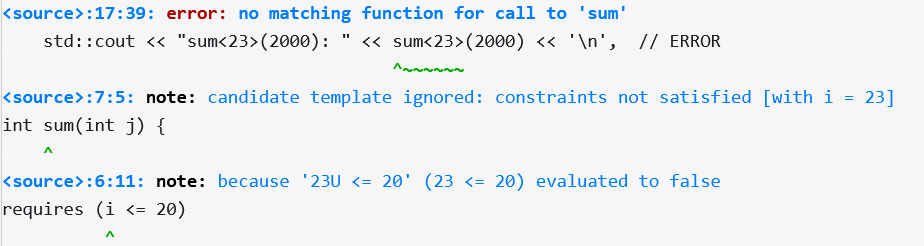
\includegraphics[width=1.0\textwidth]{content/3/chapter4/images/1-2.png}\\
requires子句中使用编译时谓词失败
\end{center}

\begin{tcolorbox}[breakable,enhanced jigsaw,colback=blue!5!white,colframe=blue!75!black,title={避免在requires子句中使用编译时谓词}]
当使用概念约束模板参数或函数模板时,应该使用命名概念或组合它们。概念属于语义范畴,而不是像i <= 20这样的语法约束。并且,为概念命名可以使其重用。
\end{tcolorbox}

\hspace*{\fill} \\ %插入空行
\noindent
\textbf{4.1.4.3\hspace{0.2cm}函数的返回类型为概念}

下面是使用概念作为返回类型的函数模板gcd和函数gcd1的定义。

\hspace*{\fill} \\ %插入空行
\noindent
\textbf{概念作为返回类型}
\begin{lstlisting}[style=styleCXX]
template<typename T>
requires std::integral<T>
std::integral auto gcd(T a, T b) {
	if( b == 0 ) return a;
	else return gcd(b, a % b);
}

std::integral auto gcd1(std::integral auto a, std::integral auto b) {
	if( b == 0 )return a;
	else return gcd1(b, a % b);
}
\end{lstlisting}

\hspace*{\fill} \\ %插入空行
\noindent
\textbf{4.1.4.4\hspace{0.2cm}概念的用例}

首先,概念是编译时谓词。编译时谓词是在编译时执行,并返回布尔值的函数。深入研究概念的各种用例前,我想先揭开概念的神秘面纱,并将它们简单地表示为在编译时返回布尔值的函数。

\hspace*{\fill} \\ %插入空行
\noindent
\textbf{4.1.4.4.1\hspace{0.2cm}编译时谓词}

概念可用于在运行时或编译时执行的控制结构中。

\hspace*{\fill} \\ %插入空行
\noindent
\textbf{概念作为编译时谓词}
\begin{lstlisting}[style=styleCXX]
// compileTimePredicate.cpp

#include <compare>
#include <iostream>
#include <string>
#include <vector>

struct Test{};

int main() {

	std::cout << '\n';

	std::cout << std::boolalpha;

	std::cout << "std::three_way_comparable<int>: "
	<< std::three_way_comparable<int> << "\n";

	std::cout << "std::three_way_comparable<double>: ";
	if (std::three_way_comparable<double>) std::cout << "True";
	else std::cout << "False";

	std::cout << "\n\n";

	static_assert(std::three_way_comparable<std::string>);

	std::cout << "std::three_way_comparable<Test>: ";
	if constexpr(std::three_way_comparable<Test>) std::cout << "True";
	else std::cout << "False";

	std::cout << '\n';

	std::cout << "std::three_way_comparable<std::vector<int>>: ";
	if constexpr(std::three_way_comparable<std::vector<int>>) std::cout << "True";
	else std::cout << "False";

	std::cout << '\n';

}
\end{lstlisting}

例子中,我使用了std::three\_way\_comparable<T>这个概念,在比较时检查T是否支持六个比较运算符。作为编译时谓词std::thre\_way\_comparable可以在运行时(第16行和第20行)或编译时使用。static\_assert(第25行)和\href{https://en.cppreference.com/w/cpp/language/if}{constepr if}(第28和34行)可在编译时进行计算。

\begin{tcblisting}{commandshell={}}
std::three_way_coparable<int>: True
std::three_way_coparable<double>: True

std::three_way_coparable<Test>: False
std::three_way_coparable<std::vector<int>>: True
\end{tcblisting}

对编译时谓词的概念进行简短的介绍之后,继续本节的概念的各种用例。这些概念的应用不是很详细,这里主要使用的是预定义概念,我将后续的章节中讨论这些概念。

\hspace*{\fill} \\ %插入空行
\noindent
\textbf{4.1.4.4.2\hspace{0.2cm}类模板}

类模板MyVector要求模板形参T是常规类型,所以T的行为类似于int。\href{https://en.cppreference.com/w/cpp/concepts/regular}{std::regular}的定义在之前有提到。

\hspace*{\fill} \\ %插入空行
\noindent
\textbf{类定义中使用概念}
\begin{lstlisting}[style=styleCXX]
// conceptsClassTemplate.cpp

#include <concepts>
#include <iostream>

template <std::regular T>
class MyVector{};

int main() {

	MyVector<int> myVec1;
	MyVector<int&> myVec2; // ERROR because a reference is not regular

}
\end{lstlisting}

因为引用非常规类型,所以第12行会出现编译错误。下面是GCC编译器错误消息的重要部分:

\begin{center}
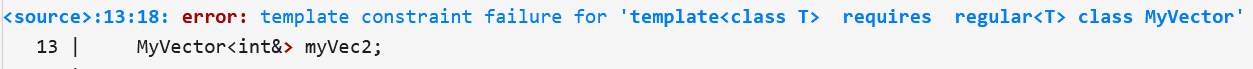
\includegraphics[width=1.0\textwidth]{content/3/chapter4/images/1-3.png}\\
引用非常规类型
\end{center}

\hspace*{\fill} \\ %插入空行
\noindent
\textbf{4.1.4.4.3\hspace{0.2cm}泛型成员函数}

这个例子中,向MyVector类添加了一个通用的push\_back成员函数。push\_back要求参数可复制。

\hspace*{\fill} \\ %插入空行
\noindent
\textbf{泛型成员函数中使用概念}
\begin{lstlisting}[style=styleCXX]
// conceptMemberFunction.cpp

#include <concepts>
#include <iostream>

struct NotCopyable {
	NotCopyable() = default;
	NotCopyable(const NotCopyable&) = delete;
};

template <typename T>
struct MyVector{
	void push_back(const T&) requires std::copyable<T> {}
};

int main() {

	MyVector<int> myVec1;
	myVec1.push_back(2020);

	MyVector<NotCopyable> myVec2;
	myVec2.push_back(NotCopyable()); // ERROR because not copyable

}
\end{lstlisting}

编译在第22行失败。因为复制构造函数声明为已删除,所以NotCopyable的实例不可复制。

\hspace*{\fill} \\ %插入空行
\noindent
\textbf{4.1.4.4.4\hspace{0.2cm}可变模板}

可变模板中可以使用概念。

\begin{lstlisting}[style=styleCXX]
// allAnyNone.cpp

#include <concepts>
#include <iostream>

template<std::integral... Args>
bool all(Args... args) { return (... && args); }

template<std::integral... Args>
bool any(Args... args) { return (... || args); }

template<std::integral... Args>
bool none(Args... args) { return not(... || args); }

int main(){

	std::cout << std::boolalpha << '\n';

	std::cout << "all(5, true, false): " << all(5, true, false) << '\n';

	std::cout << "any(5, true, false): " << any(5, true, false) << '\n';

	std::cout << "none(5, true, false): " << none(5, true, false) << '\n';

}
\end{lstlisting}

上述函数模板的定义基于折叠表达式。C++11支持可变参数模板,可以接受任意数量的模板参数,任意数量的模板参数由一个所谓的参数包保存。C++17中可以使用二进制操作符直接简化参数包,这种简化称为\href{https://www.modernescpp.com/index.php/fold-expressions}{折叠表达式}。

在本例中,逻辑和\&\&(第7行)、逻辑或||(第10行)以及逻辑或的否定(第13行)作为二元运算符。此外,all、any和none要求类型参数必须支持std::integral概念。

\begin{tcblisting}{commandshell={}}
all(5, true, false): false
any(5, true, false): true
none(5, ture, false): false
\end{tcblisting}

\hspace*{\fill} \\ %插入空行
\noindent
\textbf{4.1.4.4.5\hspace{0.2cm}重载}

\href{https://en.cppreference.com/w/cpp/iterator/advance}{std::advance}是标准模板库的算法,对给定的迭代器iter增加n个元素,根据给定迭代器的功能,可以使用不同的策略。例如,std::forward\_list支持只能朝一个方向前进的迭代器,而std::list支持双向迭代器,std::vector支持随机访问迭代器。因此,对于std::forward\_list或std::list提供的迭代器,对std::advance(iter, n)的调用必须加n倍(参见std::list的结构)耗时。这个时间复杂度不适用于std::vector提供的std::randomaccess\_iterator,数字n可以直接加到迭代器中。因此,线性时间复杂度O(n)变成了O(1)。为了区分迭代器类型,可以使用概念。conceptsOverloadingFunctionTemplates.cpp展示了这样使用概念的方式。

\begin{lstlisting}[style=styleCXX]
// conceptsOverloadingFunctionTemplates.cpp

#include <concepts>
#include <iostream>
#include <forward_list>
#include <list>
#include <vector>

template<std::forward_iterator I>
void advance(I& iter, int n){
	std::cout << "forward_iterator" << '\n';
}

template<std::bidirectional_iterator I>
void advance(I& iter, int n){
	std::cout << "bidirectional_iterator" << '\n';
}

template<std::random_access_iterator I>
void advance(I& iter, int n){
	std::cout << "random_access_iterator" << '\n';
}

int main() {

	std::cout << '\n';

	std::forward_list forwList{1, 2, 3};
	std::forward_list<int>::iterator itFor = forwList.begin();
	advance(itFor, 2);

	std::list li{1, 2, 3};
	std::list<int>::iterator itBi = li.begin();
	advance(itBi, 2);

	std::vector vec{1, 2, 3};
	std::vector<int>::iterator itRa = vec.begin();
	advance(itRa, 2);

	std::cout << '\n';
}
\end{lstlisting}

函数advance的三种重载位于std::forward\_iterator(第9行)、std::bidirectional\_iterator(第14行)和std::random\_access\_iterator(第19行)这三个概念上,编译器会选择最合适的重载。所以,对于std::forward\_list(第28行),对应的是基于std::forward\_list概念的重载;对于std::list(第32行),对应的是基于std::bidirectional\_iterator概念的重载;对于std::vector(第36行),对应的是基于std::random\_access\_iterator概念的重载。

\begin{tcblisting}{commandshell={}}
forward_iterator
bidirectional_iterator
random_access_iterator
\end{tcblisting}

std::random\_access\_iterator可以当作std::bidirectional\_iterator看待,std::bidirectional\_iterator可以当作std::forward\_iterator看待。

\hspace*{\fill} \\ %插入空行
\noindent
\textbf{4.1.4.4.6\hspace{0.2cm}特化的模板}

还可以使用概念特化的模板。

\begin{lstlisting}[style=styleCXX]
// conceptsSpecialization.cpp

#include <concepts>
#include <iostream>

template <typename T>
struct Vector {
	Vector() {
		std::cout << "Vector<T>" << '\n';
	}
};

template <std::regular Reg>
struct Vector<Reg> {
	Vector() {
		std::cout << "Vector<std::regular>" << '\n';
	}
};

int main() {

	std::cout << '\n';

	Vector<int> myVec1;
	Vector<int&> myVec2;

	std::cout << '\n';

}
\end{lstlisting}

实例化类模板时,编译器会选择最特化的一个。对于Vector<int> myVec(第24行),会选择std::regular(第13行)的偏特化模板。引用Vector<int\&> myVec2(第25行)不是std::regular类型,因此选择主模板(第6行)。

\begin{tcblisting}{commandshell={}}
Vector<std::regular>
Vector<T>
\end{tcblisting}

\hspace*{\fill} \\ %插入空行
\noindent
\textbf{4.1.4.4.7\hspace{0.2cm}使用多个概念}

目前,这些概念的使用都很简单,也可以同时使用多个概念。

\begin{lstlisting}[style=styleCXX]
template<typename Iter, typename Val>
	requires std::input_iterator<Iter>
		  && std::equality_comparable<Value_type<Iter>, Val>
Iter find(Iter b, Iter e, Val v)
\end{lstlisting}

find需要Iter迭代器与Val进行比较

\begin{itemize}
\item
迭代器必须是输入迭代器;

\item
迭代器的值类型必须与Val相同。
\end{itemize}

对迭代器的限制也可以表示为受约束的模板形参。

\begin{lstlisting}[style=styleCXX]
template<std::input_iterator Iter, typename Val>
	requires std::equality_comparable<Value_type<Iter>, Val>
Iter find(Iter b, Iter e, Val v)
\end{lstlisting}

\subsubsubsection{4.1.5\hspace{0.2cm}约束和非约束占位符}

首先,让我告诉你C++14中的一个不对称。

\hspace*{\fill} \\ %插入空行
\noindent
\textbf{4.1.5.1\hspace{0.2cm}C++14中的不对称}

我经常在课堂上进行讨论。C++14中,我们有泛型Lambda,可以使用auto。

\hspace*{\fill} \\ %插入空行
\noindent
\textbf{泛型Lambda和函数模板的比较}
\begin{lstlisting}[style=styleCXX]
// genericLambdaTemplate.cpp

#include <iostream>
#include <string>

auto addLambda = [](auto fir, auto sec){ return fir + sec; };

template <typename T, typename T2>
auto addTemplate(T fir, T2 sec){ return fir + sec; }

int main(){

	std::cout << std::boolalpha << '\n';

	std::cout << addLambda(1, 5) << " " << addTemplate(1, 5) << '\n';
	std::cout << addLambda(true, 5) << " " << addTemplate(true, 5) << '\n';
	std::cout << addLambda(1, 5.5) << " " << addTemplate(1, 5.5) << '\n';

	const std::string fir{"ge"};
	const std::string sec{"neric"};
	std::cout << addLambda(fir, sec) << " " << addTemplate(fir, sec) << '\n';

	std::cout << '\n';

}
\end{lstlisting}

泛型Lambda(第6行)和函数模板(第8行)产生相同的结果。

\begin{center}
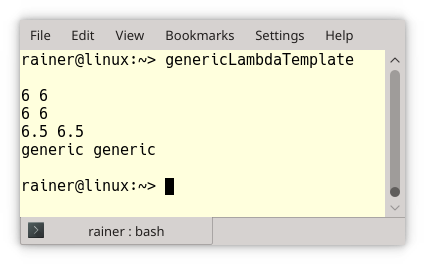
\includegraphics[width=0.6\textwidth]{content/3/chapter4/images/8.png}\\
\end{center}

泛型Lambda引入了一种定义函数模板的新方法。在课堂上,经常有人问:我们可以在函数中使用auto获取函数模板吗?C++14不行,但C++20可以。

C++20中,可以在函数声明中使用无约束占位符(auto)或有约束占位符(概念)来自动获取函数模板。规则非常简单,在每个可以使用无约束占位符auto的地方,都可以使用一个概念。我将在简写函数模板一节中进行详细说明。

\hspace*{\fill} \\ %插入空行
\noindent
\textbf{4.1.5.2\hspace{0.2cm}占位符}

\hspace*{\fill} \\ %插入空行
\noindent
\textbf{使用约束占位符}
\begin{lstlisting}[style=styleCXX]
// placeholders.cpp

#include <concepts>
#include <iostream>
#include <vector>

std::integral auto getIntegral(int val){
	return val;
}

int main(){

std::cout << std::boolalpha << '\n';

	std::vector<int> vec{1, 2, 3, 4, 5};
	for (std::integral auto i: vec) std::cout << i << " ";
	std::cout << '\n';

	std::integral auto b = true;
	std::cout << b << '\n';

	std::integral auto integ = getIntegral(10);
	std::cout << integ << '\n';

	auto integ1 = getIntegral(10);
	std::cout << integ1 << '\n';

	std::cout << '\n';

}
\end{lstlisting}

std::integral概念可以用作返回类型(第7行)、基于范围的for循环(第16行),或者用作变量b(第19行)或变量integ(第22行)的类型。为了查看auto和概念之间的对称性,第25行单独使用auto,而不是在第22行使用的std::integral auto。因此,integ1可以接受任何类型的值。

\begin{tcblisting}{commandshell={}}
1 2 3 4 5
true
10
10
\end{tcblisting}

\subsubsubsection{4.1.6\hspace{0.2cm}简写函数模板}

C++20中,可以在函数声明中使用不受约束的占位符(auto)或受约束的占位符(concept),这个函数声明会自动成为一个函数模板。

\begin{lstlisting}[style=styleCXX]
// abbreviatedFunctionTemplates.cpp

#include <concepts>
#include <iostream>

template<typename T>
requires std::integral<T>
T gcd(T a, T b) {
	if( b == 0 ) return a;
	else return gcd(b, a % b);
}

template<typename T>
T gcd1(T a, T b) requires std::integral<T> {
	if( b == 0 ) return a;
	else return gcd1(b, a % b);
}

template<std::integral T>
T gcd2(T a, T b) {
	if( b == 0 ) return a;
	else return gcd2(b, a % b);
}

std::integral auto gcd3(std::integral auto a, std::integral auto b) {
	if( b == 0 ) return a;
	else return gcd3(b, a % b);
}

auto gcd4(auto a, auto b){
	if( b == 0 ) return a;
	return gcd4(b, a % b);
}

int main() {

	std::cout << '\n';

	std::cout << "gcd(100, 10)= " << gcd(100, 10) << '\n';
	std::cout << "gcd1(100, 10)= " << gcd1(100, 10) << '\n';
	std::cout << "gcd2(100, 10)= " << gcd2(100, 10) << '\n';
	std::cout << "gcd3(100, 10)= " << gcd3(100, 10) << '\n';
	std::cout << "gcd4(100, 10)= " << gcd4(100, 10) << '\n';

	std::cout << '\n';

}
\end{lstlisting}

函数模板gcd(第6行)、gcd1(第13行)和gcd2(第19行)在使用概念的四种方式时已经介绍过了。gdc使用requires子句,gcd1使用尾部requires子句,gcd2使用约束模板参数。现在来看点新东西,函数模板gcd3有std::integral的概念作为类型参数,因此是一个具有受限类型参数的函数模板。相比之下,gcd4相当于对其类型参数,对函数模板没有限制。gcd3和gcd4中用于创建函数模板的语法,称为缩写函数模板。

\begin{tcblisting}{commandshell={}}
gcd(100, 10)= 10
gcd1(100, 10)= 10
gcd2(100, 10)= 10
gcd3(100, 10)= 10
gcd4(100, 10)= 10
\end{tcblisting}

通过下面的例子来强调这种对称性。

使用auto作为类型参数,函数add变成了一个函数模板,与同名的函数模板add等价。

\begin{lstlisting}[style=styleCXX]
template<typename T, typename T2>
auto add(T fir, T2 sec) {
	return fir + sec;
}

auto add(auto fir, auto sec) {
	return fir + sec;
}
\end{lstlisting}

相应地,由于std::integral概念的使用,sub函数等价于函数模板sub函数。

\begin{lstlisting}[style=styleCXX]
template<std::integral T, std::integral T2>
std::integral auto sub(T fir, T2 sec) {
	return fir - sec;
}

std::integral auto sub(std::integral auto fir, std::integral auto sec) {
	return fir - sec;
}
\end{lstlisting}

函数和函数模板可以是任意类型,这两种类型可以是不同的,但必须是整型。例如,使用sub(100, 10)和sub(100, true)都可以。

缩写函数模板语法中,仍然缺少一个特性:可以重载auto或概念。

\hspace*{\fill} \\ %插入空行
\noindent
\textbf{4.1.6.1\hspace{0.2cm}重载}

以下函数会在auto、std::integral概念和long类型上进行重载。

\begin{lstlisting}[style=styleCXX]
// conceptsOverloading.cpp

#include <concepts>
#include <iostream>

void overload(auto t){
	std::cout << "auto : " << t << '\n';
}

void overload(std::integral auto t){
	std::cout << "Integral : " << t << '\n';
}

void overload(long t){
	std::cout << "long : " << t << '\n';
}

int main(){

	std::cout << '\n';

	overload(3.14);
	overload(2010);
	overload(2020L);

	std::cout << '\n';

}
\end{lstlisting}

编译器选择auto(第6行)上的重载使用double,std::integral(第10行)上的重载使用int,long(第14行)上的重载使用long。

\begin{tcblisting}{commandshell={}}
auto : 3.14
Integral : 2010
long : 2020
\end{tcblisting}

\begin{tcolorbox}[breakable,enhanced jigsaw,colback=blue!5!white,colframe=blue!75!black,title={遗漏的特性:模板}]
也许在这一章的概念中遗漏了一个特性:模板。将模板引入是概念技术规范的一部分,\href{https://www.iso.org/standard/64031.html}{TS ISO/IEC TS 19217:2015}是概念的实验性实现。\href{https://en.wikipedia.org/wiki/GNU_Compiler_Collection}{GCC 6}完全实现了概念TS,除了语法上与C++20中的概念不同之外,概念TS支持一种简洁的定义模板的方式。

\hspace*{\fill} \\ %插入空行
下面的例子中,假设Integral是一个概念。

\hspace*{\fill} \\ %插入空行
\noindent
\textbf{概念TS中的模板介绍}
\begin{lstlisting}[style=styleCXX]
Integral{T}
Integral gcd(T a, T b){
	if( b == 0 ){ return a; }
	else{
		return gcd(b, a % b);
	}
}

Integral{T}
class ConstrainedClass{};
\end{lstlisting}

上面的这个小代码片段,以两种方式引入了模板。首先,定义一个带有约束模板参数的函数模板;其次,定义带有约束模板参数的类模板。引入模板有一个限制,只能将其用于有约束的模板参数(concept),而不能用于无约束的模板参数(auto)。这种不对称性可以通过定义一个总是返回true的概念轻松搞定:

\hspace*{\fill} \\ %插入空行
\noindent
\textbf{Generic概念的实现}
\begin{lstlisting}[style=styleCXX]
template<typename T>
concept bool Generic(){
	return true;
}
\end{lstlisting}

不要着急,我在示例中使用概念TS语法来定义泛型概念。C++20的语法会简洁一些。在定义概念一节中可以了解更多的C++20语法细节。
\end{tcolorbox}

\subsubsubsection{4.1.7\hspace{0.2cm}预定义的概念}

“不要白费力气”的黄金法则同样适用于概念。\href{https://isocpp.github. io/CppCoreGuidelines/CppCoreGuidelines}{C++核心指南}对这条规则的定义非常清楚:\textit{T.11:只要可能,就使用标准概念}。因此,我想给出一个重要的预定义概念的概述,这里会有意地忽略特殊或辅助类型的概念。

所有预定义的概念在最新的C++20工作草案\href{https://isocpp.org/files/papers/N4860.pdf}{N4860}中都有详细描述,找到它们是一个相当大的挑战!大部分概念都在第18章(概念库)和第24章(范围库)中。另外,第17章(语言支持库)、第20章(通用实用程序库)、第23章(迭代器库)和第26章(数字库)中有一些概念。C++20草案N4860还提供了所有库概念的索引,并展示了如何实现这些概念。

\hspace*{\fill} \\ %插入空行
\noindent
\textbf{4.1.7.1\hspace{0.2cm}语言支持库}

本节讨论一个有趣的概念——three\_way\_comparable,支持三向比较运算符,在头文件<compare>中定义。

更正式地说,设a和b是类型为t的值。只有在以下情况下,这些值才支持three\_way\_comparable:

\begin{tcblisting}{commandshell={}}
• (a <=> b == 0) == bool(a == b) is true
• (a <=> b != 0) == bool(a != b) is true
• ((a <=> b) <=> 0) and (0 <=> (b <=> a)) are equal
• (a <=> b < 0) == bool(a < b) is true
• (a <=> b > 0) == bool(a > b) is true
• (a <=> b <= 0) == bool(a <= b) is true
• (a <=> b >= 0) == bool(a >= b) is true
\end{tcblisting}

\hspace*{\fill} \\ %插入空行
\noindent
\textbf{4.1.7.2\hspace{0.2cm}概念库}

最常用的概念可以在概念库中找到,在<concepts>头文件中定义。

\hspace*{\fill} \\ %插入空行
\noindent
\textbf{4.1.7.2.1\hspace{0.2cm}语言相关的概念}

本节有大约15个概念,这些概念表示类型、类型分类和基本类型属性之间的关系。其实现通常直接基于\href{https://en.cppreference.com/w/cpp/header/type_traits}{类型特性库}中的相应函数。若有必要,我会提供额外的解释。

\begin{itemize}
\item
same\_as

\item
derived\_from

\item
convertible\_to

\item
common\_reference\_with: common\_reference\_with<T, U>必须定义良好,T和U必须可以转换为引用类型C,其中C与common\_reference\_t<T, U>相同

\item
common\_with: 类似于common\_reference\_with,但是common类型C与common\_type\_t<T, U>相同,并且可能不是引用类型

\item
assignable\_from

\item
swappable
\end{itemize}

\hspace*{\fill} \\ %插入空行
\noindent
\textbf{4.1.7.2.2\hspace{0.2cm}算术的概念}

\begin{itemize}
\item
integral

\item
signed\_integral

\item
unsigned\_integral

\item
floating\_point
\end{itemize}

该标准对算术概念的定义很简单:

\begin{lstlisting}[style=styleCXX]
template<class T>
concept integral = is_integral_v<T>;

template<class T>
concept signed_integral = integral<T> && is_signed_v<T>;

template<class T>
concept unsigned_integral = integral<T> && !signed_integral<T>;

template<class T>
concept floating_point = is_floating_point_v<T>;
\end{lstlisting}

\hspace*{\fill} \\ %插入空行
\noindent
\textbf{4.1.7.2.3\hspace{0.2cm}生命周期的概念}

\begin{itemize}
\item
destructible

\item
constructible\_from

\item
default\_constructible

\item
move\_constructible

\item
copy\_constructible
\end{itemize}

\hspace*{\fill} \\ %插入空行
\noindent
\textbf{4.1.7.2.4\hspace{0.2cm}比较的概念}

\begin{itemize}
\item
equality\_comparable

\item
totally\_ordered
\end{itemize}

学习数学时会了解:对于类型T的值a、b和c,若以下描述成立,则T类型为totally\_ordered(全序关系)

\begin{itemize}
\item
bool(a < b)、bool(a > b)或bool(a == b)中的一个为真

\item
bool(a < b)和bool(b < c),则bool(a < c)

\item
bool(a > b) == bool(b < a)

\item
bool(a <= b) == !bool(b < a)

\item
bool(a >= b) == !bool(a < b)
\end{itemize}

\hspace*{\fill} \\ %插入空行
\noindent
\textbf{4.1.7.2.5\hspace{0.2cm}对象的概念}

\begin{itemize}
\item
movable

\item
copyable

\item
semiregular

\item
regular
\end{itemize}

以下是这四个概念的定义:

\begin{lstlisting}[style=styleCXX]
template<class T>
concept movable = is_object_v<T> && move_constructible<T> &&
					assignable_from<T&, T> && swappable<T>;

template<class T>
concept copyable = copy_constructible<T> && movable<T> &&
					assignable_from<T&, T&> &&
					assignable_from<T&, const T&> && assignable_from<T&, const T>;

template<class T>
concept semiregular = copyable<T> && default_initializable<T>;

template<class T>
concept regular = semiregular<T> && equality_comparable<T>;
\end{lstlisting}

我必须补充几点。可移动的概念要求T的is\_object\_v<T>条件成立。根据类型特性is\_object<T>的定义,T可以是标量、数组、联合体或者类。

定义概念部分还实现了半常规和常规的概念。不太正式地说,半常规类型的行为类似于int类型;而常规类型的行为也类似于int类型,并且可以使用==操作符进行比较。

\hspace*{\fill} \\ %插入空行
\noindent
\textbf{4.1.7.2.6\hspace{0.2cm}可调用的概念}

\begin{itemize}
\item
invocable

\item
regular\_invocable:类型建模为可调用且保持相等,并且不修改函数参数;保持相等,说明在给定相同的输入时会产生相同的输出

\item
predicate:若类型对可调用对象建模并返回布尔值,则可对谓词建模
\end{itemize}

\hspace*{\fill} \\ %插入空行
\noindent
\textbf{4.1.7.3\hspace{0.2cm}通用工具库}

本章在标准中只有特殊的内存概念,因此在这里不提及它们。

\hspace*{\fill} \\ %插入空行
\noindent
\textbf{4.1.7.4\hspace{0.2cm}迭代器库}

迭代器库有许多重要的概念,在<iterator>头文件中定义。下面是迭代器的类别:

\begin{itemize}
\item
input\_iterator

\item
output\_iterator

\item
forward\_iterator

\item
bidirectional\_iterator

\item
random\_access\_iterator

\item
contiguous\_iterator
\end{itemize}

这六类迭代器对应于各自的迭代器概念。下表提供了两条有趣的信息。对于三个最突出的迭代器类别,该表显示了它们的属性和相关的标准库容器。

\begin{table}[H]
\centering
\begin{tabular}{lll}
\textbf{迭代器类别}   & \textbf{属性} & \textbf{相应容器}                                                                                     \\ \hline
std::forward\_iterator &
\begin{tabular}[c]{@{}l@{}}++It,It++,*It\\ It==It2, It!=It2\end{tabular} &
\begin{tabular}[c]{@{}l@{}}std::unordered\_set\\ std::unordered\_map\\ std::unordered\_multiset\\ std::unordered\_multimap\\ std::forward\_list\end{tabular} \\ \hline
std::bidirectional\_iterator & -{}-It,It-{}-           & \begin{tabular}[c]{@{}l@{}}std::set\\ std::map\\ std::multiset\\ std::multimap\\ std::list\end{tabular} \\ \hline
std::random\_access\_iterator &
\begin{tabular}[c]{@{}l@{}}It{[}i{]}\\ It += n, It -= n\\ It + n, It - n,\\ n + It,\\ It - It2,\\ It \textless It2, It \textless{}= It2\\ It \textless It2, It \textgreater{}= It2\end{tabular} &
\begin{tabular}[c]{@{}l@{}}std::array\\ std::vector\\ std::deque\\ std::string\end{tabular}
\end{tabular}
\end{table}

以下关系成立:

\begin{itemize}
\item
随机访问迭代器是双向迭代器,双向迭代器是前向迭代器。

\item
连续迭代器是一种随机访问迭代器,要求容器的元素连续存储在内存中。
\end{itemize}

所以std::array,std::vector和std::string支持连续迭代器,但不包括std::deque。

\hspace*{\fill} \\ %插入空行
\noindent
\textbf{4.1.7.4.1\hspace{0.2cm}算法的概念}

\begin{itemize}
\item
permutable:元素可直接重排序

\item
mergeable:可以将已排序的序列合并到输出序列中

\item
sortable:可以将一个序列排列成有序序列
\end{itemize}

\hspace*{\fill} \\ %插入空行
\noindent
\textbf{4.1.7.5\hspace{0.2cm}范围库}

范围库包含对范围和视图特性至关重要的概念,类似于迭代器库中的概念,定义在<ranges>头文件中。

\hspace*{\fill} \\ %插入空行
\noindent
\textbf{4.1.7.5.1\hspace{0.2cm}范围}

\begin{itemize}
\item
range:范围指定可以遍历的一组项,提供了一个开始迭代器和一个结束哨兵。当然,STL容器也有范围。
\end{itemize}

对于std::ranges::range还可以进一步的细化。

\begin{itemize}
\item
input\_range:指定一个范围,其迭代器类型满足input\_iterator(例如,可以从开始迭代到结束至少一次)

\item
output\_range:指定迭代器类型满足output\_iterator的范围

\item
forward\_range:指定一个范围,其迭代器类型满足forward\_iterator(可以从开始到结束迭代多次)

\item
bidirectional\_range:指定迭代器类型满足bidirectional\_iterator的范围(可以向前和向后迭代不止一次)

\item
random\_access\_range:指定迭代器类型满足random\_access\_iterator的范围(可以在常量时间内使用索引操作符[]跳访问任意元素)

\item
contiguous\_range:指定一个范围,其迭代器类型满足contiguous\_iterator(元素连续存储在内存中)
\end{itemize}

标准模板库的每个容器都支持特定的范围,支持的范围指定了其迭代器的功能。

\begin{table}[H]
\centering
\begin{tabular}{lll}
\textbf{迭代器类型}        & \textbf{属性} & \textbf{相应容器}                                                                                     \\ \hline
std::ranges::input\_range &
\begin{tabular}[c]{@{}l@{}}++It,It++,*It\\ It==It2, It!=It2\end{tabular} &
\begin{tabular}[c]{@{}l@{}}std::unordered\_set\\ std::unordered\_map\\ std::unordered\_multiset\\ std::unordered\_multimap\\ std::forward\_list\end{tabular} \\ \hline
std::ranges::bidirectional\_range & -{}-It,It-{}-           & \begin{tabular}[c]{@{}l@{}}std::set\\ std::map\\ std::multiset\\ std::multimap\\ std::list\end{tabular} \\ \hline
std::ranges::random\_access\_range &
\begin{tabular}[c]{@{}l@{}}It{[}i{]}\\ It += n, It -= n\\ It + n, It - n,\\ n + It,\\ It - It2,\\ It \textless It2, It \textless{}= It2\\ It \textless It2, It \textgreater{}= It2\end{tabular} &
std::deque \\ \hline
std::ranges::contiguous\_range &
\begin{tabular}[c]{@{}l@{}}It{[}i{]}\\ It += n, It -= n\\ It + n, It - n,\\ n + It,\\ It - It2,\\ It \textless It2, It \textless{}= It2\\ It \textless It2, It \textgreater{}= It2\end{tabular} &
\begin{tabular}[c]{@{}l@{}}std::array\\ std::vector\\ std::string\end{tabular}
\end{tabular}
\end{table}

若容器支持std::ranges::continuous\_range概念,则支持表中提到的所有概念,如std::ranges::random\_access\_range,std::ranges::bidirectional\_range和std::ranges::input\_range。对于其他范围同理。

\hspace*{\fill} \\ %插入空行
\noindent
\textbf{4.1.7.5.2\hspace{0.2cm}视图}

std::ranges::view通常是应用在一个范围上,并用其执行一些操作。视图不拥有数据,视图用于复制、移动或赋值的时间恒定。下面引用Eric Niebler的range-v3实现(是C++20范围的基础):“视图是范围的组合适配,随着视图的迭代,这种适配的功能会慢慢地发挥其功效。”

\hspace*{\fill} \\ %插入空行
\noindent
\textbf{4.1.7.6\hspace{0.2cm}数值库}

数值库提供了uniform\_random\_bit\_generator的概念,该概念定义在头文件<random>中。类型G的uniform\_random\_bit\_generator g必须返回均分布的无符号整数,类型为G的均匀随机位生成器g必须支持成员函数G::min和G::max。

\subsubsubsection{4.1.8\hspace{0.2cm}自定义概念}

当在C++20中没有合适的预定义的概念时,可以自定义概念。在本节中,我将定义几个概念,使用CamelCase语法将它们与预定义的概念区别开来。因此,我的带符号整型的概念命名为signeintegral,而C++标准的概念为signed\_integral。

定义概念的语法很简单:

\begin{lstlisting}[style=styleCXX]
template <template-parameter-list>
concept concept-name = constraint-expression;
\end{lstlisting}

概念定义从关键字template开始,并有一个模板参数列表。第二行更有趣,使用关键字概念,后面跟着概念名称和约束表达式。

约束表达式可以是:

\begin{itemize}
\item
概念或编译时谓词的逻辑组合

\begin{itemize}
\item
逻辑组合可以由连接(\&\&)、析取(||)或否定(!)

\item
编译时谓词是在编译时返回布尔值的可调用对象
\end{itemize}

\item
需求表达式
\begin{itemize}
\item
简单的需求

\item
类型的需求

\item
复合的需求

\item
嵌套的需求
\end{itemize}
\end{itemize}

接下来的两节中,将演示定义概念的各种方法。

\hspace*{\fill} \\ %插入空行
\noindent
\textbf{4.1.8.1\hspace{0.2cm}其他概念和编译时谓词的组合}

可以使用连接词(\&\&)和析取词(||)组合概念和编译时谓词。构建逻辑组合时,可以使用感叹号(!)否定。因为\href{https://en.cppreference.com/w/cpp/header/type_traits}{类型特性库}有许多编译时谓词,所以具备了使用构建强大概念所需的工具。

\hspace*{\fill} \\ %插入空行
\begin{tcolorbox}[breakable,enhanced jigsaw,colback=red!5!white,colframe=red!75!black,title={不要递归地定义概念或尝试约束它们}]

概念的递归定义无效:

\hspace*{\fill} \\ %插入空行
\noindent
\textbf{递归地定义概念}
\begin{lstlisting}[style=styleCXX]
template<typename T>
concept Recursive = Recursive<T*>;
\end{lstlisting}

GCC编译器在这种情况下抱怨'Recursive'没有在此作用域中声明。

\hspace*{\fill} \\ %插入空行
当尝试约束概念(例如下面的代码片段)时,GCC编译器会明确地提示概念不能约束。

\hspace*{\fill} \\ %插入空行
\noindent
\textbf{约束概念}
\begin{lstlisting}[style=styleCXX]
template<typename T>
concept AlwaysTrue = true;

template<typename T>
requires AlwaysTrue<T>
concept Error = true;
\end{lstlisting}

\end{tcolorbox}

我们先从Integral、signeintegral和unsigneintegral概念开始。

\begin{lstlisting}[style=styleCXX]
template <typename T>
concept Integral = std::is_integral<T>::value;

template <typename T>
concept SignedIntegral = Integral<T> && std::is_signed<T>::value;

template <typename T>
concept UnsignedIntegral = Integral<T> && !SignedIntegral<T>;
\end{lstlisting}

我使用类型特性函数\href{https://en.cppreference.com/w/cpp/types/is_integral}{std::is\_integral}来定义Integral概念(第2行)。由于函数std::is\_signed,将Integral概念改进为SignedIntegral概念(第4行)。最后,对SignedIntegral概念进行否定,得到了UnsignedIntegral概念(第7行)。

Okay,我们来试试看。

\begin{lstlisting}[style=styleCXX]
// SignedUnsignedIntegrals.cpp

#include <iostream>
#include <type_traits>

template <typename T>
concept Integral = std::is_integral<T>::value;

template <typename T>
concept SignedIntegral = Integral<T> && std::is_signed<T>::value;

template <typename T>
concept UnsignedIntegral = Integral<T> && !SignedIntegral<T>;

void func(SignedIntegral auto integ) {
	std::cout << "SignedIntegral: " << integ << '\n';
}

void func(UnsignedIntegral auto integ) {
	std::cout << "UnsignedIntegral: " << integ << '\n';
}

int main() {

	std::cout << '\n';

	func(-5);
	func(5u);

	std::cout << '\n';

}
\end{lstlisting}

使用简化的函数模板语法重载概念SignedIntegral(第15行)和UnsignedIntegral(第19行)上的函数func。编译器选择预期的重载:

\begin{tcblisting}{commandshell={}}
SignedIntegral: -5
UnsignedIntegral: 5
\end{tcblisting}

出于完整性的原因,会下面的算术概念中使用析取。

\begin{lstlisting}[style=styleCXX]
template <typename T>
concept Arithmetic = std::is_integral<T>::value || std::is_floating_point<T>::value;
\end{lstlisting}

\hspace*{\fill} \\ %插入空行
\noindent
\textbf{4.1.8.2\hspace{0.2cm}需求表达式}

因为需求表达式,现在可以定义功能强大的概念。需求表达式有如下形式:

\begin{lstlisting}[style=styleCXX]
requires (parameter-list(optional)) {requirement-seq}
\end{lstlisting}

\begin{itemize}
\item
参数列表:以逗号分隔的参数列表,例如:在函数声明中

\item
需求序列:由简单需求、类型需求、复合需求或嵌套需求组成
\end{itemize}

\hspace*{\fill} \\ %插入空行
\noindent
\textbf{4.1.8.2.1\hspace{0.2cm}简单的需求}

下面是概念Addable的简单需求:

\begin{lstlisting}[style=styleCXX]
template<typename T>
concept Addable = requires (T a, T b) {
	a + b;
};
\end{lstlisting}

Addable的概念要求两个相同类型T可以进行加法a + b。

\begin{tcolorbox}[breakable,enhanced jigsaw,colback=blue!5!white,colframe=blue!75!black,title={避免使用匿名概念}]

可以定义一个匿名概念并直接使用,但请避免这样做。这会使得代码难以阅读,并且无法重用相应的概念。

\hspace*{\fill} \\ %插入空行
\noindent
\textbf{一个匿名概念,用于添加两个概念}
\begin{lstlisting}[style=styleCXX]
template<typename T>
	requires requires (T x) { x + x; }
T add1(T a, T b) { return a + b; }
\end{lstlisting}

函数模板自定义了概念,Add1在require子句中使用需求表达式。匿名概念等同于前面定义的概念Addable,下面使用命名概念Addable的函数模板add2也是如此。

\hspace*{\fill} \\ %插入空行
\noindent
\textbf{使用Addable概念}
\begin{lstlisting}[style=styleCXX]
template<Addable T>
T add2(T a, T b) { return a + b; }
\end{lstlisting}

概念应该对一般情况进行封装,并为它们提供一个自解释的名称以便重用。这对于维护代码非常重要。匿名概念读起来更像模板参数的语法约束。

\end{tcolorbox}

\hspace*{\fill} \\ %插入空行
\noindent
\textbf{4.1.8.2.2\hspace{0.2cm}类型的需求}

类型的需求中,必须使用关键字typename和类型名。

\begin{lstlisting}[style=styleCXX]
template<typename T>
concept TypeRequirement = requires {
	typename T::value_type;
	typename Other<T>;
};
\end{lstlisting}

TypeRequirement概念要求类型T有一个嵌套的成员value\_type,并且类模板Other可以用T实例化。让我们试试这个:

\begin{lstlisting}[style=styleCXX]
#include <iostream>
#include <vector>

template <typename>
struct Other;

template <>
struct Other<std::vector<int>> {};

template<typename T>
concept TypeRequirement = requires {
	typename T::value_type;
	typename Other<T>;
};

int main() {

	TypeRequirement auto myVec= std::vector<int>{1, 2, 3};

}
\end{lstlisting}

表达式TypeRequirement auto myVec = std::vector<int>{1,2,3}(第18行)有效。\href{https://en.cppreference.com/w/cpp/container/vector}{std::vector}有一个内部成员value\_type(第12行),类模板Other可以实例化std::vector<int>(第13行)。

\hspace*{\fill} \\ %插入空行
\noindent
\textbf{4.1.8.2.3\hspace{0.2cm}复合需求}

复合需求有这样的形式

\begin{lstlisting}[style=styleCXX]
{expression} noexcept(optional) return-type-requirement(optional);
\end{lstlisting}

除了简单的需求外,复合需求还可以有\href{https://en.cppreference.com/w/cpp/language/noexcept_spec}{noexcept说明符}和关于其返回类型的需求。

下面的示例中演示了在Equal概念中,使用复合需求。

\begin{lstlisting}[style=styleCXX]
// conceptsDefinitionEqual.cpp

#include <concepts>
#include <iostream>

template<typename T>
concept Equal = requires(T a, T b) {
	{ a == b } -> std::convertible_to<bool>;
	{ a != b } -> std::convertible_to<bool>;
};

bool areEqual(Equal auto a, Equal auto b){
	return a == b;
}

struct WithoutEqual{
	bool operator==(const WithoutEqual& other) = delete;
};

struct WithoutUnequal{
	bool operator!=(const WithoutUnequal& other) = delete;
};

int main() {

	std::cout << std::boolalpha << '\n';
	std::cout << "areEqual(1, 5): " << areEqual(1, 5) << '\n';

	/*

	bool res = areEqual(WithoutEqual(), WithoutEqual());
	bool res2 = areEqual(WithoutUnequal(), WithoutUnequal());

	*/

	std::cout << '\n';

}
\end{lstlisting}

Equal概念(第6行)要求其类型参数T支持相等和不相等操作符。此外,两个操作符都必须返回一个可转换为布尔值的值。当然,int支持Equal概念,但这并不适用于WithoutEqual(第16行)和WithoutUnequal(第20行)类型。因此,当使用WithoutEqual类型时(第31行),在使用GCC编译器时,会得到以下错误消息。

\begin{center}
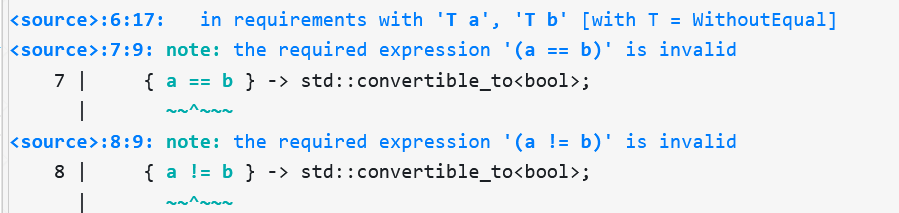
\includegraphics[width=0.8\textwidth]{content/3/chapter4/images/1-4.png}\\
WithoutEqual不匹配Equal概念
\end{center}

\hspace*{\fill} \\ %插入空行
\noindent
\textbf{4.1.8.2.4\hspace{0.2cm}嵌套需求}

嵌套需求的形式

\begin{lstlisting}[style=styleCXX]
requires constraint-expression;
\end{lstlisting}

嵌套需求用于指定类型参数上的需求。

下面是定义概念unsigneintegral的另一种方法(参见概念和谓词的逻辑组合):

\begin{lstlisting}[style=styleCXX]
// nestedRequirements.cpp

#include <type_traits>

template <typename T>
concept Integral = std::is_integral<T>::value;

template <typename T>
concept SignedIntegral = Integral<T> && std::is_signed<T>::value;

// template <typename T>
// concept UnsignedIntegral = Integral<T> && !SignedIntegral<T>;

template <typename T>
concept UnsignedIntegral = Integral<T> &&
requires(T) {
	requires !SignedIntegral<T>;
};

int main() {

	UnsignedIntegral auto n = 5u; // works
	// UnsignedIntegral auto m = 5; // compile time error, 5 is a signed literal

}
\end{lstlisting}

第14行使用signeintegral概念,嵌套需求来细化Integral概念。老实说,第11行中注释掉的概念unsigneintegral阅读起来更方便。

下一节中的有序概念演示了嵌套需求的使用。

\subsubsubsection{4.1.9\hspace{0.2cm}应用}

前面的章节中,回答了关于概念的两个基本问题:“如何使用概念?“和“如何定义你的概念?”

本节中,将应用这些理论知识来定义更高级的概念,如Ordering、SemiRegular和Regular。

\hspace*{\fill} \\ %插入空行
\noindent
\textbf{4.1.9.1\hspace{0.2cm}Equal和Ordering的概念}

我已经在Haskell的类型的层次结构中介绍了概念的漫长历史:

\begin{center}
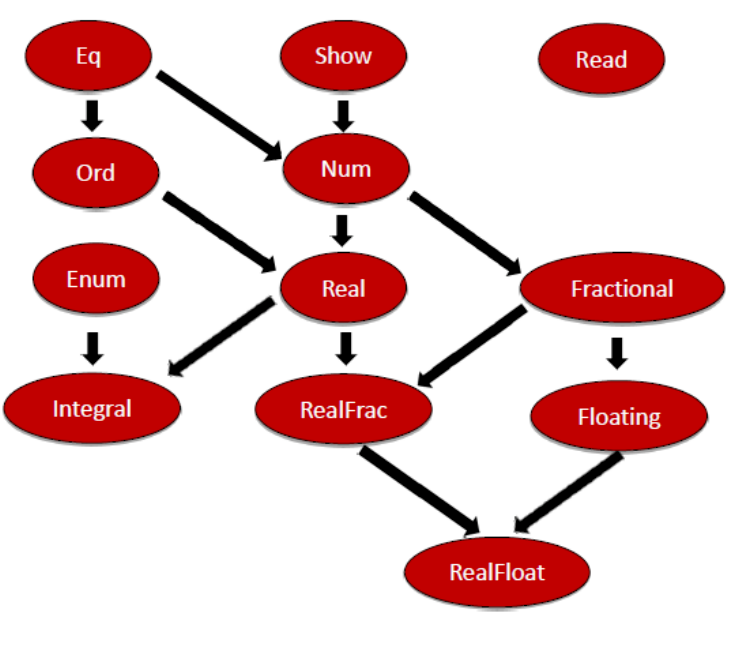
\includegraphics[width=0.6\textwidth]{content/3/chapter4/images/9.png}\\
Haskell类型的层次结构
\end{center}

类层次结构表明类型Ord是类型Eq的细化,Haskell优雅地表达了这一点。

\hspace*{\fill} \\ %插入空行
\noindent
\textbf{Haskell类型层次结构的一部分}
\begin{lstlisting}[style=styleCXX]
class Eq a where
	(==) :: a -> a -> Bool
	(/=) :: a -> a -> Bool

class Eq a => Ord a where
	compare :: a -> a -> Ordering
	(<) :: a -> a -> Bool
	(<=) :: a -> a -> Bool
	(>) :: a -> a -> Bool
	(>=) :: a -> a -> Bool
	max :: a -> a -> a
\end{lstlisting}

每个类型a支持类型类Eq(第1行),必须支持等式(第2行)和不等式(第3行)。支持类型类Ord的每个类型a都必须支持类型类Eq(在第5行中,(Eq a => Ord a)。此外,类型a必须支持四个比较操作符,以及compare和max函数(第6-11行)。

能否用C++20中的概念来表达Haskell在类型Eq和Ord之间的关系?为了简单起见,这里忽略Haskell的compare和max函数。

\hspace*{\fill} \\ %插入空行
\noindent
\textbf{4.1.9.1.1\hspace{0.2cm}排序概念}

有了需求表达式,排序概念的定义看起来与Haskell中类型类ord的定义相似。

\begin{lstlisting}[style=styleCXX]
template <typename T>
concept Ordering =
	Equal<T> &&
	requires(T a, T b) {
		{ a <= b } -> std::convertible_to<bool>;
		{ a < b } -> std::convertible_to<bool>;
		{ a > b } -> std::convertible_to<bool>;
		{ a >= b } -> std::convertible_to<bool>;
	};
\end{lstlisting}

排序概念在底层使用了嵌套的需求。类型T若支持Equal概念,则支持排序概念,此外还支持四个比较运算符。

\hspace*{\fill} \\ %插入空行
\noindent
\textbf{排序概念的定义和使用}
\begin{lstlisting}[style=styleCXX]
// conceptsDefinitionOrdering.cpp

#include <concepts>
#include <iostream>
#include <unordered_set>

template<typename T>
concept Equal =
	requires(T a, T b) {
		{ a == b } -> std::convertible_to<bool>;
		{ a != b } -> std::convertible_to<bool>;
	};


template <typename T>
concept Ordering =
	Equal<T> &&
	requires(T a, T b) {
		{ a <= b } -> std::convertible_to<bool>;
		{ a < b } -> std::convertible_to<bool>;
		{ a > b } -> std::convertible_to<bool>;
		{ a >= b } -> std::convertible_to<bool>;
	};

template <Equal T>
bool areEqual(const T& a, const T& b) {
	return a == b;
}

template <Ordering T>
T getSmaller(const T& a, const T& b) {
	return (a < b) ? a : b;
}

int main() {

	std::cout << std::boolalpha << '\n';

	std::cout << "areEqual(1, 5): " << areEqual(1, 5) << '\n';

	std::cout << "getSmaller(1, 5): " << getSmaller(1, 5) << '\n';

	std::unordered_set<int> firSet{1, 2, 3, 4, 5};
	std::unordered_set<int> secSet{5, 4, 3, 2, 1};

	std::cout << "areEqual(firSet, secSet): " << areEqual(firSet, secSet) << '\n';

	// auto smallerSet = getSmaller(firSet, secSet);

	std::cout << '\n';

}
\end{lstlisting}

函数模板areEqual(第25行)要求实参a和b具有相同的类型并支持Equal概念,函数模板getsmall(第30行)要求两个参数都支持有序概念。当然,像1和5这样的整数可以同时匹配这两个概念,而\href{https://en.cppreference.com/w/cpp/container/unordered_set}{std::unordered\_set}并不匹配有序概念。

因此,我将第48行注释掉。

\begin{tcblisting}{commandshell={}}
areEqual(1, 5): false
getSmaller(1, 5): 1
areEqual(firSet, secSet): true
\end{tcblisting}

接下来,当编译第48行会发生什么?GCC编译器明确指出std::unordered\_set不是函数模板getsmall的有效参数。

\begin{center}
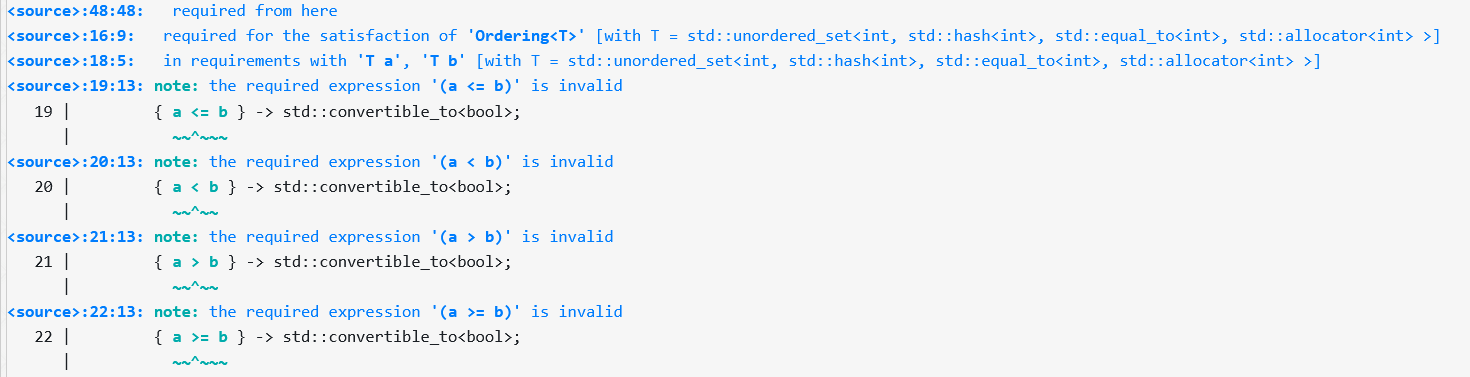
\includegraphics[width=1.0\textwidth]{content/3/chapter4/images/1-5.png}\\
函数模板getsmall的使用错误
\end{center}

排序概念已经是C++20标准的一部分。

\begin{itemize}
\item
std::three\_way\_comparable:等价于上面提出的排序概念

\item
std::three\_way\_comparable\_with:允许比较不同类型的值;例如:1.0 < 1.0f
\end{itemize}

C++20中,可以使用三向比较操作符,也称为宇宙飞船操作符<=>。我将在三向比较运算符的章节中介绍它。

\hspace*{\fill} \\ %插入空行
\noindent
\textbf{4.1.9.2\hspace{0.2cm}半常规(SemiRegular)和常规(Regular)的概念}

想要在C++生态系统中定义一个工作良好的类型时,应该定义一个“行为像int型”的类型。形式上,具体类型应该是常规类型在本节中,来定义半常规和常规概念。

半常规和常规是C++中的基本思想。抱歉,我应该说概念。例如,在《C++核心指南》中的解释\href{http://isocpp.github.io/CppCoreGuidelines/CppCoreGuidelines#Rt-regular}{T.46:要求模板参数至少是半常规和常规类型}。现在,只剩下一个重要的问题需要回答:什么是常规类型或半常规类型?在讨论之前,先给出结论:

\begin{itemize}
\item
常规类型“行为类似于int型”,可以复制,并且复制操作的结果独立于原始操作,具有相同的值。
\end{itemize}

更正式一点。常规类型也是半常规类型,让我们开始吧。


\begin{tcolorbox}[breakable,enhanced jigsaw,colback=blue!5!white,colframe=blue!75!black,title={常规类型}]

\href{https://en.wikipedia.org/wiki/Alexander_Stepanov}{Alexander Stepanov},标准模板库的设计者,定义了术语常规类型和半常规类型。根据他的说法,若一个类型支持这些函数,那么它就是常规类型

\begin{itemize}
\item
复制构造

\item
赋值

\item
等式

\item
析构

\item
全序
\end{itemize}

复制构造意味着默认构造,等式构造意味着不相等。Stepanov定义上述需求时,C++中还没有移动语义。Alexander Stepanov和\href{https://www.mcjones.org/paul/}{Paul McJones}合著的书\href{http://elementsofprogramming.com/}{Elements of Programming}专门介绍了常规类型。

\end{tcolorbox}

\hspace*{\fill} \\ %插入空行
\noindent
\textbf{4.1.9.2.1\hspace{0.2cm}半常规概念}

一个半常规的X型必须支持六大函数,并且可交换。六大函数包括:

\begin{itemize}
\item
默认构造函数:
\begin{lstlisting}[style=styleCXX]
X()
\end{lstlisting}

\item
复制构造函数:
\begin{lstlisting}[style=styleCXX]
X(const X&)
\end{lstlisting}

\item
复制赋值操作符:
\begin{lstlisting}[style=styleCXX]
X& operator = (const X&)
\end{lstlisting}

\item
移动构造函数:
\begin{lstlisting}[style=styleCXX]
X(X&&)
\end{lstlisting}

\item
移动赋值操作符:
\begin{lstlisting}[style=styleCXX]
X& operator = (X&&)
\end{lstlisting}

\item
析构函数:
\begin{lstlisting}[style=styleCXX]
~X()
\end{lstlisting}
\end{itemize}

此外,X必须是可交换的: swap(X\&, X\&)

\href{https://en.cppreference.com/w/cpp/header/type_traits}{类型特性库}中定义了相应概念。这里,我定义了类型特征isSemiRegular,然后用它来定义概念SemiRegular。

\begin{lstlisting}[style=styleCXX]
template<typename T>
struct isSemiRegular: std::integral_constant<bool,
								std::is_default_constructible<T>::value &&
								std::is_copy_constructible<T>::value &&
								std::is_copy_assignable<T>::value &&
								std::is_move_constructible<T>::value &&
								std::is_move_assignable<T>::value &&
								std::is_destructible<T>::value &&
								std::is_swappable<T>::value >{};


template<typename T>
concept SemiRegular = isSemiRegular<T>::value;
\end{lstlisting}

类型特性isSemiRegular(第1行)是当所有的类型特性到六大函数(第3-8行)和类型特质std::is\_swappable(第9行)都满足时实现的。定义SemiRegular概念的剩余步骤,就是使用类型特征isSemiRegular(第13行)。

我们继续解读Regular概念。

\hspace*{\fill} \\ %插入空行
\noindent
\textbf{4.1.9.2.2\hspace{0.2cm}常规概念}

我们已经完成了对Regular概念的定义。除了SemiRegular概念的需求外,Regular概念还要求类型具有相等的可比性。我已经在需求表达式一节中定义了Equal概念。因此,已经完成了,只需要把Equal和SemiRegular这两个概念组合起来就可以了。

\begin{lstlisting}[style=styleCXX]
template<typename T>
concept Regular = Equal<T> &&
					SemiRegular<T>;
\end{lstlisting}

现在,如何在C++20中定义相应的概念std::semiregular和std::regular?

\hspace*{\fill} \\ %插入空行
\noindent
\textbf{4.1.9.2.3\hspace{0.2cm}std::semiregular和std::regular}

C++20使用了现有类型特征和概念,定义了std::semiregular和std::regular概念。

\begin{lstlisting}[style=styleCXX]
template<class T>
concept movable = is_object_v<T> && move_constructible<T> &&
					assignable_from<T&, T> && swappable<T>;

template<class T>
concept copyable = copy_constructible<T> && movable<T> &&
					assignable_from<T&, T&> &&
					assignable_from<T&, const T&> && assignable_from<T&, const T>;

template<class T>
concept semiregular = copyable<T> && default_initializable<T>;

template<class T>
concept regular = semiregular<T> && equality_comparable<T>;
\end{lstlisting}

std::regular概念的定义类似于Regular概念,std::semiregular概念可以与基本概念相结合,如std::copyable和std::moveable。std::movable概念基于类型特征函数\href{https://en.cppreference.com/w/cpp/types/is_object}{std::is\_object}。cppreference.com还提供了编译时谓词的可能实现。

\begin{lstlisting}[style=styleCXX]
template< class T>
struct is_object : std::integral_constant<bool,
					std::is_scalar<T>::value ||
					std::is_array<T>::value ||
					std::is_union<T>::value ||
					std::is_class<T>::value> {};
\end{lstlisting}

若类型是标量、数组、联合体或类,则它是对象。

结束本节之前,我想使用用户定义的概念Regular和C++20的概念std::regular。regularSemiRegular.cpp完成了这项工作。

\hspace*{\fill} \\ %插入空行
\noindent
\textbf{概念Regular和SemiRegular的应用}
\begin{lstlisting}[style=styleCXX]
// regularSemiRegular.cpp

#include <concepts>
#include <vector>
#include <type_traits>

template<typename T>
struct isSemiRegular: std::integral_constant<bool,
		std::is_default_constructible<T>::value &&
		std::is_copy_constructible<T>::value &&
		std::is_copy_assignable<T>::value &&
		std::is_move_constructible<T>::value &&
		std::is_move_assignable<T>::value &&
		std::is_destructible<T>::value &&
		std::is_swappable<T>::value >{};

template<typename T>
concept SemiRegular = isSemiRegular<T>::value;

template<typename T>
concept Equal =
	requires(T a, T b) {
		{ a == b } -> std::convertible_to<bool>;
		{ a != b } -> std::convertible_to<bool>;
};

template<typename T>
concept Regular = Equal<T> &&
				SemiRegular<T>;

template <Regular T>
void behavesLikeAnInt(T) {
	// ...
}

template <std::regular T>
void behavesLikeAnInt2(T) {
	// ...
}

struct EqualityComparable { };
bool operator == (EqualityComparable const&,
				  EqualityComparable const&) {
	return true;
}

struct NotEqualityComparable { };

int main() {

	int myInt{};
	behavesLikeAnInt(myInt);
	behavesLikeAnInt2(myInt);

	std::vector<int> myVec{};
	behavesLikeAnInt(myVec);
	behavesLikeAnInt2(myVec);

	EqualityComparable equComp;
	behavesLikeAnInt(equComp);
	behavesLikeAnInt2(equComp);

	NotEqualityComparable notEquComp;
	behavesLikeAnInt(notEquComp);
	behavesLikeAnInt2(notEquComp);

}
\end{lstlisting}

我将前面代码片段中的所有部分放在一起定义Regular概念(第27行)。函数模板behavesLikeAnInt(第31行)和behavesLikeAnInt2(第36行)检查参数是否“行为像int”。使用用户自定义的概念Regular和C+20的概念std::regular来建立条件。所以,类型EqualityComparable(第41行)支持相==操作符,但类型NotEqualityComparable(第47行)不支持。在两个函数中(第64行和第65行)使用NotEqualityComparable类型是这个程序中最有趣的部分。

虽然目前处于概念实现的早期阶段,这里就比较一下新的GCC和MSVC编译器的错误消息。

\begin{itemize}
\item
GCC

我在\href{https://godbolt.org/}{Compiler Explorer}上使用当前的GCC 10.2命令行参数-std=c++20。当使用用户自定义的Regular(第64行)概念时,会出现编译错误,这里只展示比较重要的错误消息:

\begin{center}
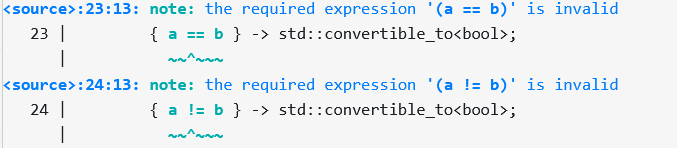
\includegraphics[width=1.0\textwidth]{content/3/chapter4/images/1-6.png}\\
\end{center}

C++20概念std::regular更加全面。因此,第65行中的调用给出了一个更全面的错误消息:

\begin{center}
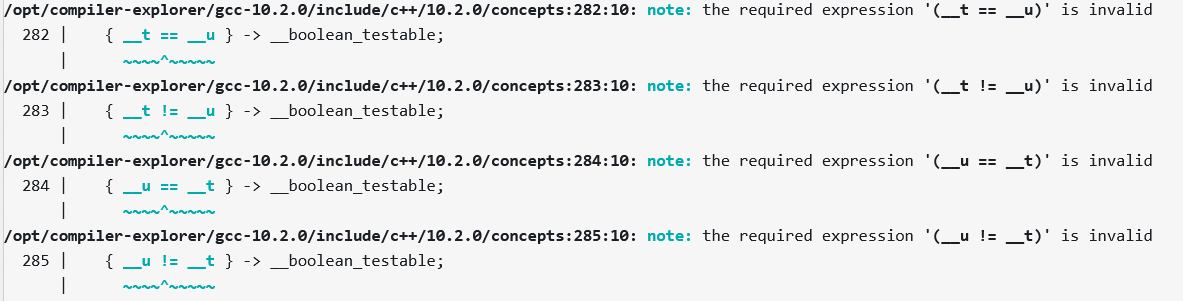
\includegraphics[width=1.0\textwidth]{content/3/chapter4/images/1-7.png}\\
\end{center}

\item
MSVC

MSVC编译器给出的错误信息就不太具体了。

\begin{center}
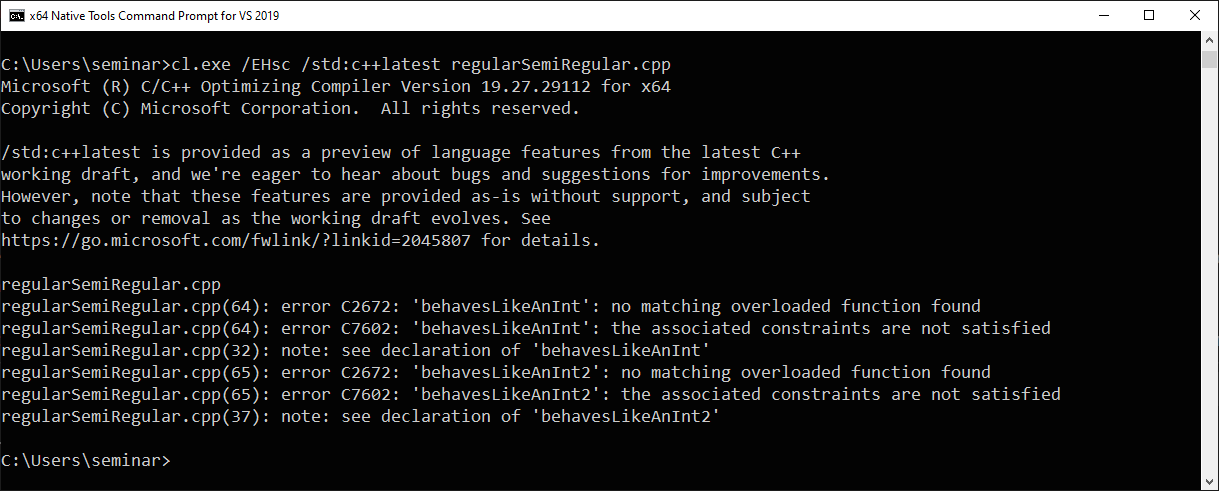
\includegraphics[width=1.0\textwidth]{content/3/chapter4/images/10.png}\\
使用std::regular概念时出现错误消息
\end{center}

从截图中看到的,编译器为19.27.29112的x64版本,并且使用了命令行参数/EHSC和/std:c++latest。

\end{itemize}

\hspace*{\fill} \\ %插入空行
\begin{tcolorbox}[breakable,enhanced jigsaw,colback=blue!5!white,colframe=blue!75!black,title={常规类型}]

这里我想表达一下我自己的观点。首先,我陈述事实,然后得出结论。这些事实都是基于本章所述内容。那么,哪些论点支持改进,哪些论点支持革命呢?

\hspace*{\fill} \\ %插入空行
\noindent
\textbf{改进派}

\begin{itemize}
\item
概念促进在更高抽象级别上使用泛型代码。

\item
当编译模板失败时,概念会给出可以理解的错误消息,提供了无法通过\href{https://en.cppreference.com/w/cpp/header/type_traits}{type-traits库}、\href{https://en.cppreference.com/w/cpp/language/sfinae}{SFINAE}和\href{https://en.cppreference.com/w/cpp/language/static_assert}{static\_assert}实现的功能。

\item
auto是一种不受约束的占位符。C++20中,可以将概念用作有约束的占位符。

\item
C++14中,可以使用泛型Lambda定义函数模板。
\end{itemize}

\noindent
\textbf{革命派}

\begin{itemize}
\item
概念促进在更高抽象级别上使用泛型代码。

\item
概念允许我们验证模板需求。当然,也可以通过组合\href{https://en.cppreference.com/w/cpp/header/type_traits}{type-traits库}、\href{https://en.cppreference.com/w/cpp/language/sfinae}{SFINAE}和\href{https://en.cppreference.com/w/cpp/language/static_assert}{static\_assert}来实现模板参数的验证,但是这种技术太高级了,不能将其视为通用解决方案。

\item
有了简写的函数模板语法,从而模板定义得到了根本性的改进。

\item
概念表示语义类别,而不是语法约束。我们不需要像Addable这样的概念,要求类型支持加法操作符,而应该考虑数字概念,其中数字是一个语义类别,例如:相等或有序。
\end{itemize}

\hspace*{\fill} \\ %插入空行
\noindent
\textbf{我的结论}

关于概念是该改进稳步向前,还是进行革命性的飞跃,有很多争论。争端主要是因为语义分类,我是站在革命派这一边的。诸如“数”、“相等”或“排序”等概念让我想起了\href{https://en.wikipedia.org/wiki/Plato}{Plato}的思想世界。若我们现在可以在这样的语义中进行编程,这将具有革命性意义。
\end{tcolorbox}

\begin{tcolorbox}[breakable,enhanced jigsaw,colback=mygreen!5!white,colframe=mygreen!75!black,title={总结}]
\begin{itemize}
\item
定义在特定类型或类型参数上的函数或类有一组问题,概念通过对类型参数施加语义约束来解决这些问题。

\item
概念可以应用在requires子句中,约束的模板参数,或在缩写函数模板中。

\item
概念是编译时谓词,可用于各种模板。也可以重载概念,使用概念特化模板,将概念用于成员函数或可变参数模板。

\item
因为C++20和概念,不受约束占位符(auto)和受约束占位符(concept)的使用方式统一了。无论何时使用auto,都可以使用C++20中的概念。

\item
新的简化的函数模板语法,使得定义函数模板变得更加简单。

\item
定义自己的概念之前,请先研究C++20标准中丰富的预定义概念集。定义概念时,可以使用两种技术:结合概念和编译时谓词,或者使用需求表达式。
\end{itemize}
\end{tcolorbox}

\newpage

















